In the previous chapter we introduced the FastSRM algorithm, a framework to
efficiently compute shared responses from the full brain data of multiple
subjects. In this chapter, we
investigate the practical benefits of FastSRM on synthetic and real fMRI data.
FastSRM reduces the fitting time
and memory requirements are reduced considerably, making it possible to compute
shared responses using a laptop in a reasonable amount of time even on
datasets that do not hold in RAM. The efficiency of FastSRM allows us to apply
SRM on a large number of subjects. As an example, we apply FastSRM on 647
subjects from the CamCAN dataset and study how the mixing matrices of the SRM
model are predictive of age.


\section{Comparing Fitting time and performance of FastSRM and
  SRM on synthetic data}
We generate synthetic data $\xb_i$ according to the model of Probabilistic SRM.
The parameters $\sigma_i$, $A_i$ and $\Sigma_s$ are generated randomly. We sample the value of the subject specific noise level from a normal
distribution: $\sigma_i \sim \Ncal(0, 0.1)$. The mixing matrices $A_i$
are obtained by sampling their coefficient from a standardized normal distribution.
Lastly, the covariance of the shared response $\Sigma_s$ is diagonal and the
diagonal values are obtained by sampling from a Dirichlet distribution with
parameter $(1 \dots 1)$.
We set the number of voxels to $v=125~000$, the number of subjects to $m=10$ and
the number of components to $p=50$. We generate $n=1000$ samples.

We benchmark deterministic SRM, probabilistic
SRM and their FastSRM counterparts in terms of fitting time and performance.
Algorithms are designated by the atlas they use and therefore SRM algorithms described in
section~\ref{sec:probabilisticsrm} and~\ref{sec:deterministicsrm} are refered to
as \emph{None} because no atlas is used and FastSRM algorithms will have the
label \emph{Optimal}. Note that it would be possible to use FastSRM with sub-optimal
atlases (there exists a wide variety of atlases
available~\cite{schaefer2017local, bellec2010multi, mensch2018extracting}) but
without any guarantees that the performance are the same as SRM.


We use a number of iterations between 1 and 100 and report the performance,
fitting time and a measure of convergence. In FastSRM, we do not compute the
unmixing matrices but only the shared response.
We measure the performance of an algorithm by computing the error between the true component $S \in \RR^{p, n}$ and
the predicted component $\hat{S} \in \RR^{p, n}$ using the quantity:
$\mathrm{mse}(\hat{S}, S) = min_{A \in \RR^{p, p}} \|A \hat{S} - S \|^2_F =  \|S
\hat{S}^{\dagger}\hat{S} - S \|^2_F$. This way of measuring errors is
insensitive to the indeterminacies in DetSRM.
We measure the fitting time in seconds.
Lastly, we measure convergence by computing the gradient $\ell_{\infty}$ norm in
case of DetSRM given by $\max(\mathrm{abs}(G))$ where $G$ is the gradient and
use the distance between consecutive values of the loss for ProbSRM.

Results are plotted in figure~\ref{fig:srm:synthetic_gradient}. 
We empirically see that the optimal approach is equivalent to using no atlas in
terms of performance. This is predicted by the theory in the previous chapter
where we demonstrate that these two algorithms yield exactly the same output from the same input.
% %
% Among approximate methods, the projection
% method yields the best results but are quite far away from optimal results.
% %
In general probabilistic methods give much better results than their deterministic
counterpart. This shows the superiority of likelihood based methods.
In terms of fitting time, FastSRM is about a thousand time faster than SRM after
100 iterations. When no atlas is used, the number
of iterations has a very strong impact on performance while it has a small impact
when the optimal atlas is used. 
Lastly, looking at the convergence curves, we see that even after $100$ iterations, algorithms did
not fully converge. This means that in practice a much larger number of
iterations is needed which would yield even a higher difference in fitting time
between methods using no atlas and methods using the optimal atlas.

\begin{figure}
  \centering
  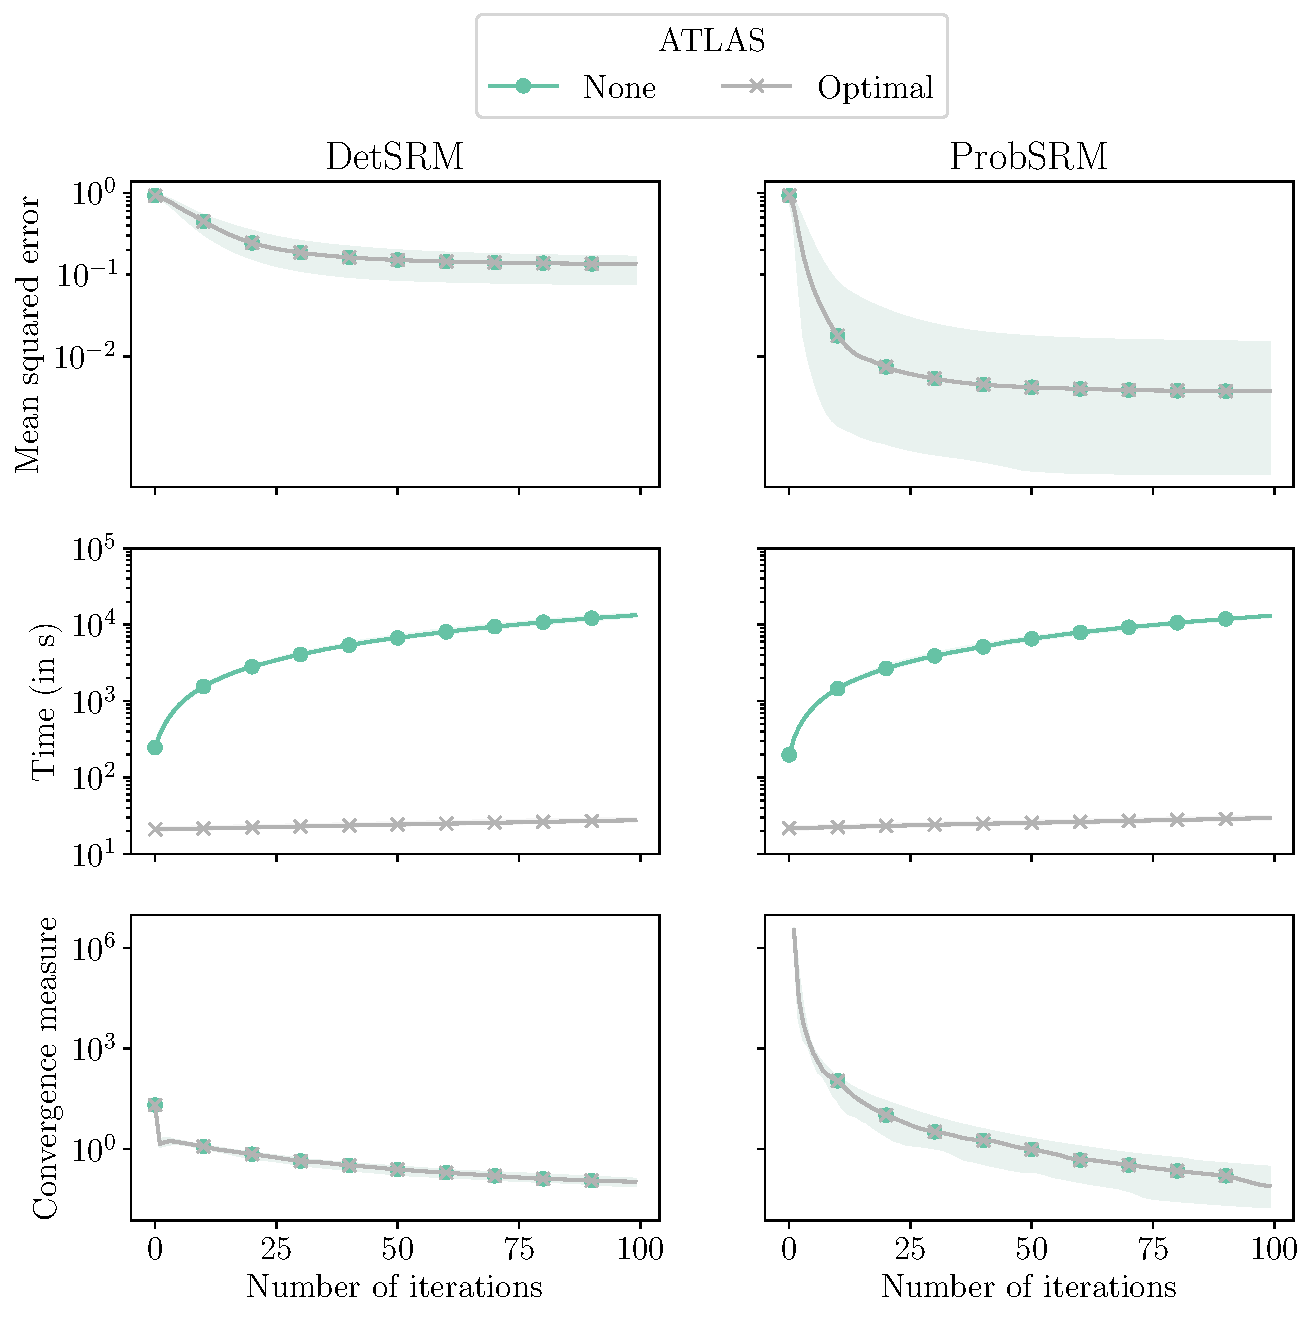
\includegraphics[width=\textwidth]{figures/srm/synthetic_gradient.pdf}
  \caption{\textbf{Benchmark of SRM algorithms on synthetic data: } Performance,
    fitting time and convergence of SRM algorithms in the deterministic (left)
    or probabilistic (right) case.  As expected, when optimal atlases are used,
    the performance is the same as if no atlas is used but the fitting time is
    much lower. This is even more pronounced when the number of iterations is
    high (and looking at convergence curves, we see that more iterations could
    be performed to be closer to a stationary point).}
  \label{fig:srm:synthetic_gradient}
\end{figure}

\section{Experiments on fMRI data}
We evaluate the performance of FastSRM on three fMRI datasets of subjects
exposed to naturalistic stimuli: Sherlock, Forrest and CamCAN (more details
about these datasets are available in section~\ref{srm:datasets:fmri}).
\subsection{Comparing fitting time, memory usage and performance on a
  timesegment matching experiment}
\label{sec:timesegment_expe}
\label{timesegment_expe}
The timesegment matching experiment is first introduced
in~\cite{chen2015reduced}.
In a nutshell, the time-segment matching accuracy measures the similarity between two multivariate time-series by trying to localize a time-segment in one time-series by correlation with the other.
In the context of movie watching, this measure has a lot of sense: if we split
the movies in scenes and compute a representation per scene and per subject, it makes
sense to assume that different subjects watching the movie would still have closer representation of the same scenes than of different scenes.
This explains why timesegment matching is a standard evaluation of SRM-like methods also used in  \cite{guntupalli2018computational}, \cite{Nastase741975} or
\cite{zhang2016searchlight}.

We now describe more precisely the experimental design.
We split the runs into a train and test set. After fitting the model on the
training set, we apply the unmixing matrices $W_i=A_i^{-1}$ of each subject on the test set yielding individual components matrices. We estimate the shared responses by averaging the individual components of each subjects but one.  We select a target time-segment (9 consecutive timeframes) in the shared responses and try to localize the corresponding time segment in the components of the left-out subject using a maximum-correlation classifier.
The time-segment is said to be
correctly classified if the correlation between the sample and target
time-segment is higher than with any other time-segment (partially overlapping time windows are excluded).
% 
We use 5-Fold cross-validation across runs: the training set contains 80\% of the runs and the test set 20\%, and repeat the experiment using all possible choices for left-out subjects. 
% 
The mean accuracy is reported in Figure~\ref{fig:srm:timesegment} (bottom).  When the
optimal atlas is used, the accuracy is the same as when no atlas is used but
the fitting time is reduced by a factor 10 to 100 and so is the memory usage.
% 

\begin{figure}
  \centering
  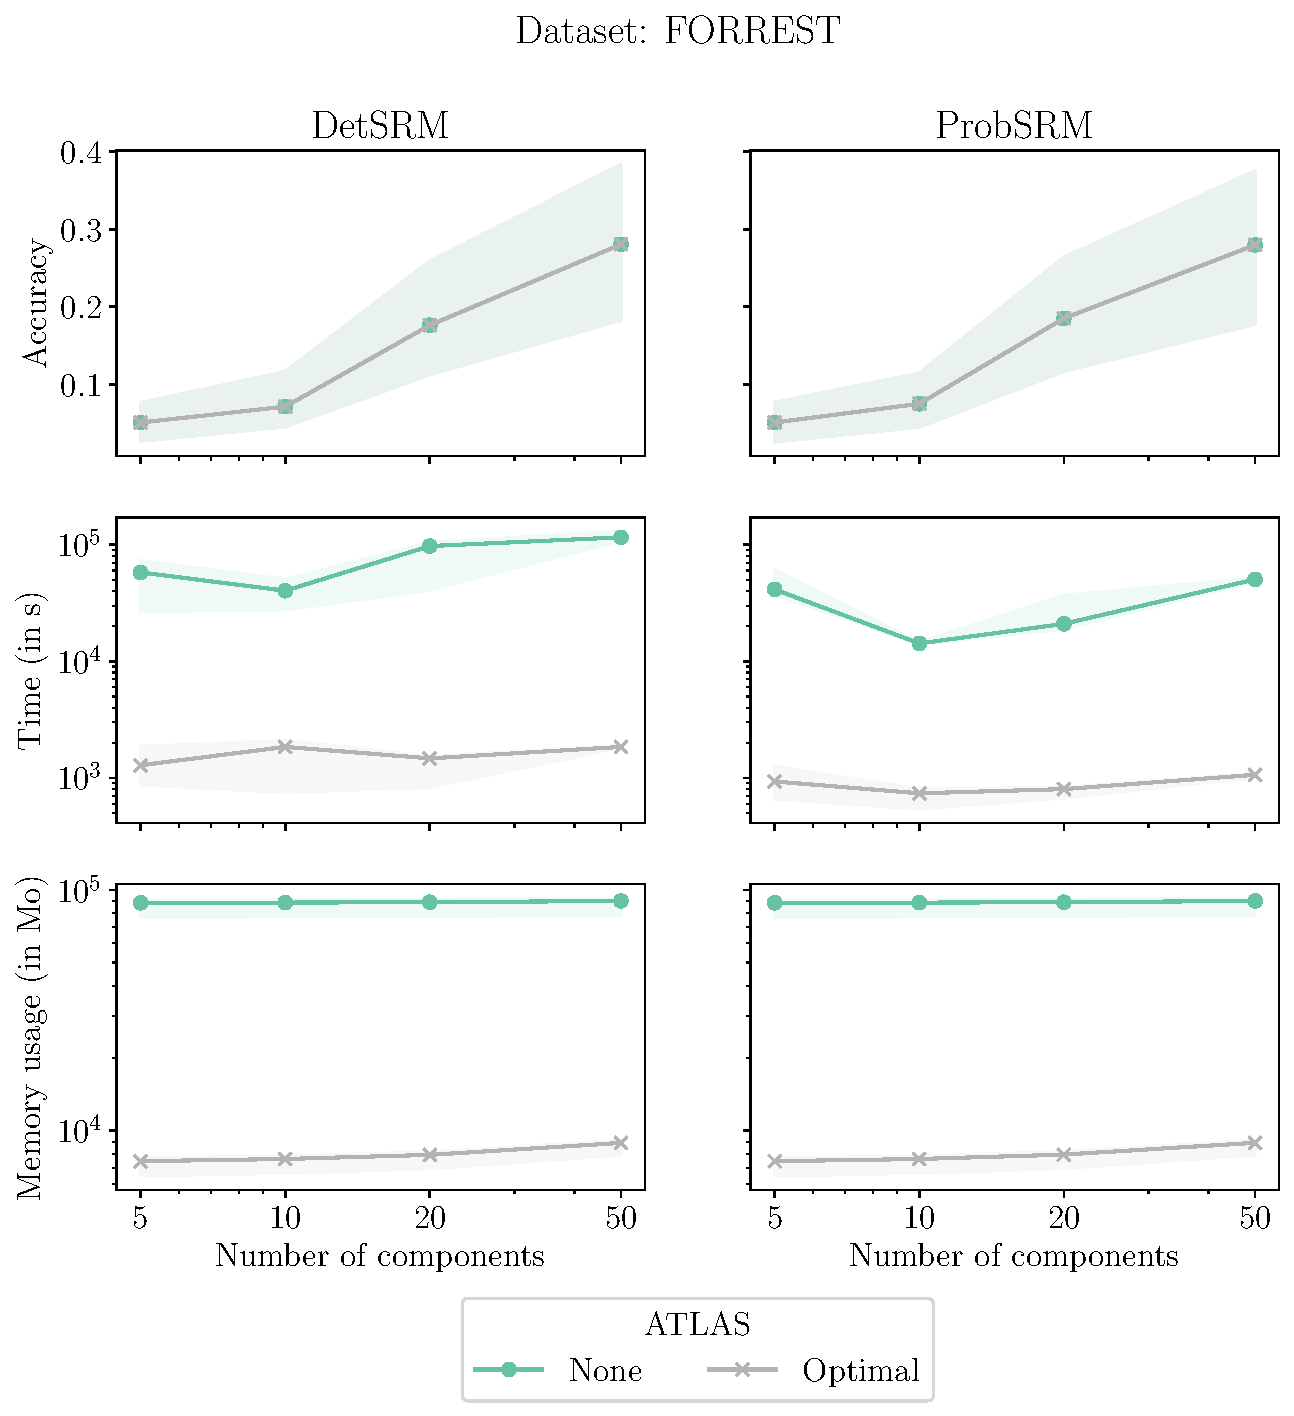
\includegraphics[width=0.8\textwidth]{figures/srm/timesegment_matching_forrest.pdf}
  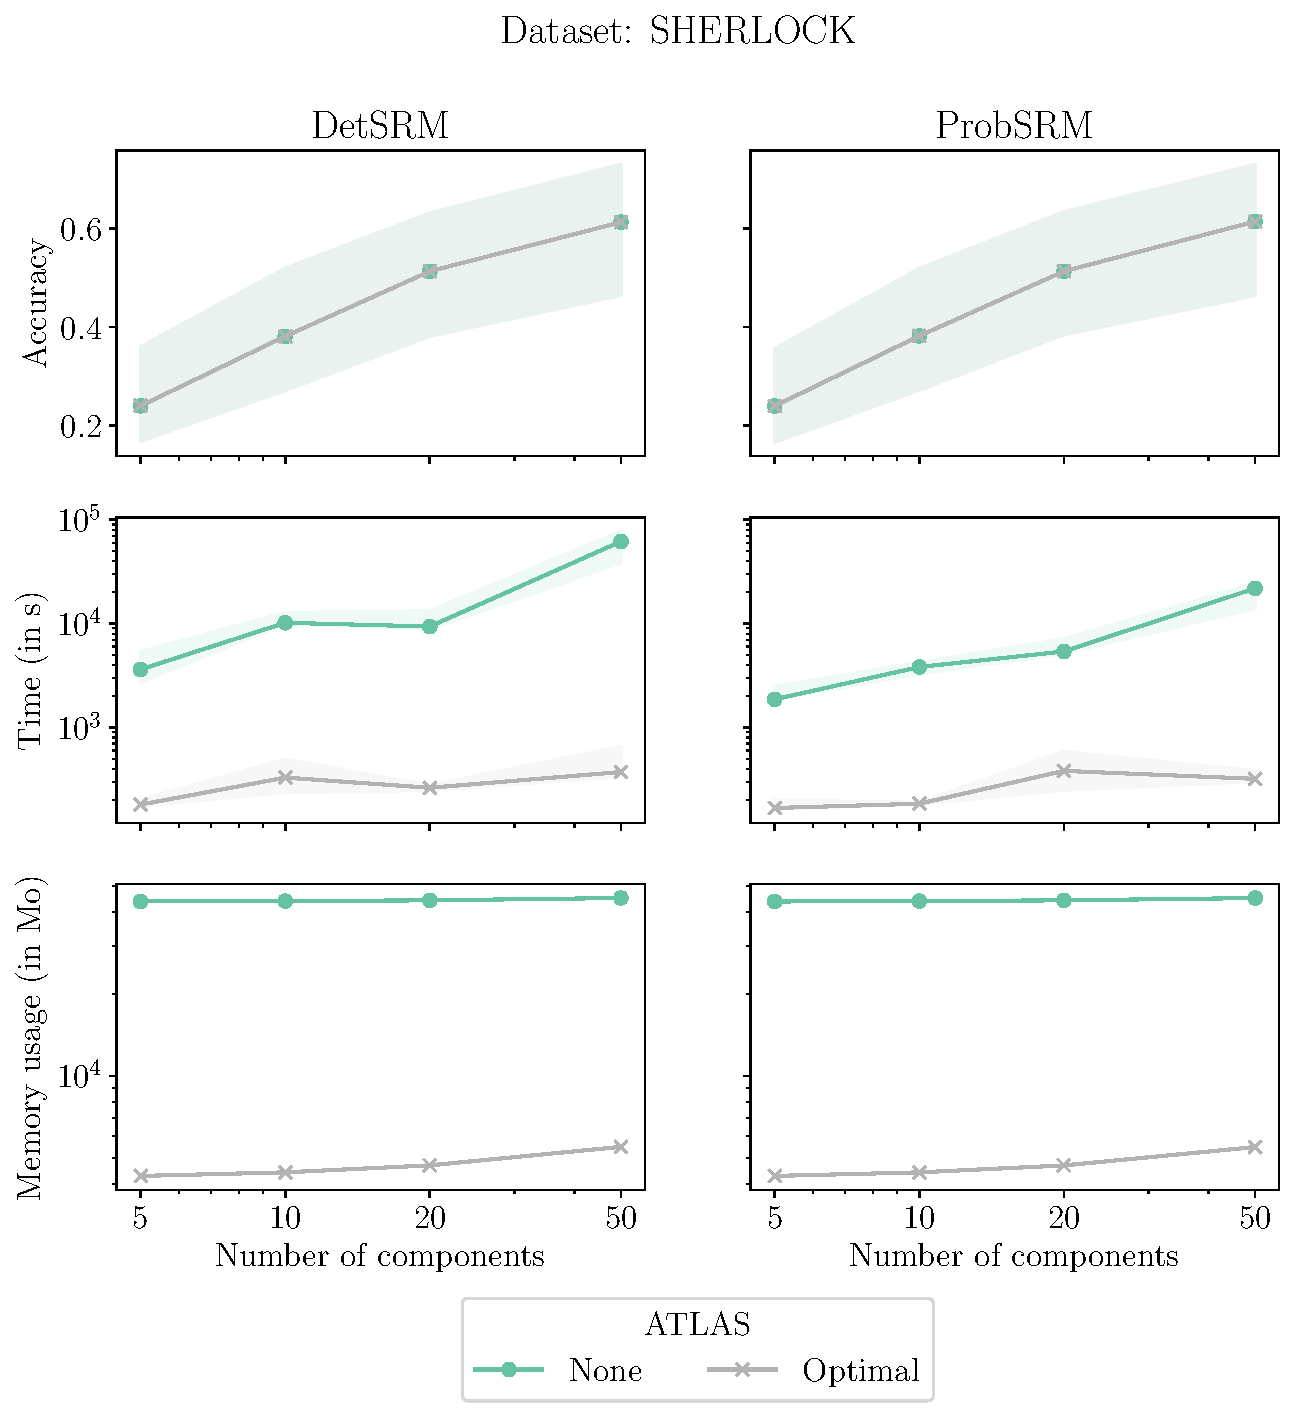
\includegraphics[width=0.8\textwidth]{figures/srm/timesegment_matching_sherlock.pdf}
  \caption{\textbf{Benchmark of SRM algorithms on fMRI data} (top) Timesegment
    matching accuracy (middle) Fitting time (bottom) Memory usage. When the
    optimal atlas is used, the accuracy is the same as when no atlas is used but
  the fitting time is reduced by a factor 10 to 100 and so is the memory usage.}
  \label{fig:srm:timesegment}
\end{figure}


We would like to highlight here that these experiments are not exactly the same
as in~\cite{chen2015reduced} as we use full brain data and they use regions of
interest. However, the code used for this experiment is very similar to the tutorial in \url{https://brainiak.org/tutorials/11-SRM/}.

\subsection{Predict age from spatial components}
Because FastSRM is fast and memory efficient, it enables large-scale analysis of fMRI recordings of subjects exposed to the same naturalistic stimuli.
% 
We use all 647 subjects of the CamCAN dataset and demonstrate the usefulness of FastSRM by showing that the spatial components that it extracts from movie watching data are predictive of age.
% 
A key asset of FastSRM is that these spatial components can be visualized and therefore provide meaningful insights. 

Note that while it is possible to do the same study using probabilistic SRM, the
table in figure~\ref{fig:predict_age} shows that the memory usage of
probabilistic SRM is 10x more important than FastSRM, almost reaching the memory
limits of our cluster and is about 200x slower. FastSRM could be
easily used with a much higher number of subjects while keeping the computation
time and memory requirements reasonable while this would be impossible with ProbSRM.

We now describe our age prediction pipeline.
Functionally matched spatial components $A_i$ are obtained using FastSRM.
%
They are divided into two groups (train and test data) where the train set contains 80\% of the data and the test set 20\%.
%
Within the train set we split again our data into two groups: the first group is
used to train one Ridge model per spatial components to predict age, the second group is used to train a Random Forest to predict age from Ridge predictions. This way of stacking models is similar to the pipeline used in \cite{rahim2017joint}.
%
We use 5 fold cross validation to split the train set (so that the number of samples used to train the Random Forest is the number of elements in the train set).
%
Then the train set is used to train one Ridge model per spatial component.
%
On the test set each Ridge model makes a prediction and the predictions are aggregated using the Random Forest model.
%
An illustration of the process is available in Figure~\ref{fig:experiment_age_prediction}. 

In each Ridge model, the coefficient that determines the level of l2 penalization is set by generalized cross validation, an efficient form of leave-one-out cross validation.

The train and test sets are chosen randomly. In Figure~\ref{fig:predict_age}, we report the average mean absolute error (MAE) on the test set averaged over the 5 splits.
FastSRM predicts age with an accuracy much better than chance resulting in a
mean absolute error (MAE) of $7.5$ years. Note that this is far from being the
most accurate method. Using a combination of different modalities, it is
possible to obtain a MAE of approximately $4.5$
years~\cite{engemann2019combining}. However, as will be shown in the next
paragraph, our method extracts a set of
components specific to each individual making it more interpretable than other approaches.

\begin{figure}
\centering
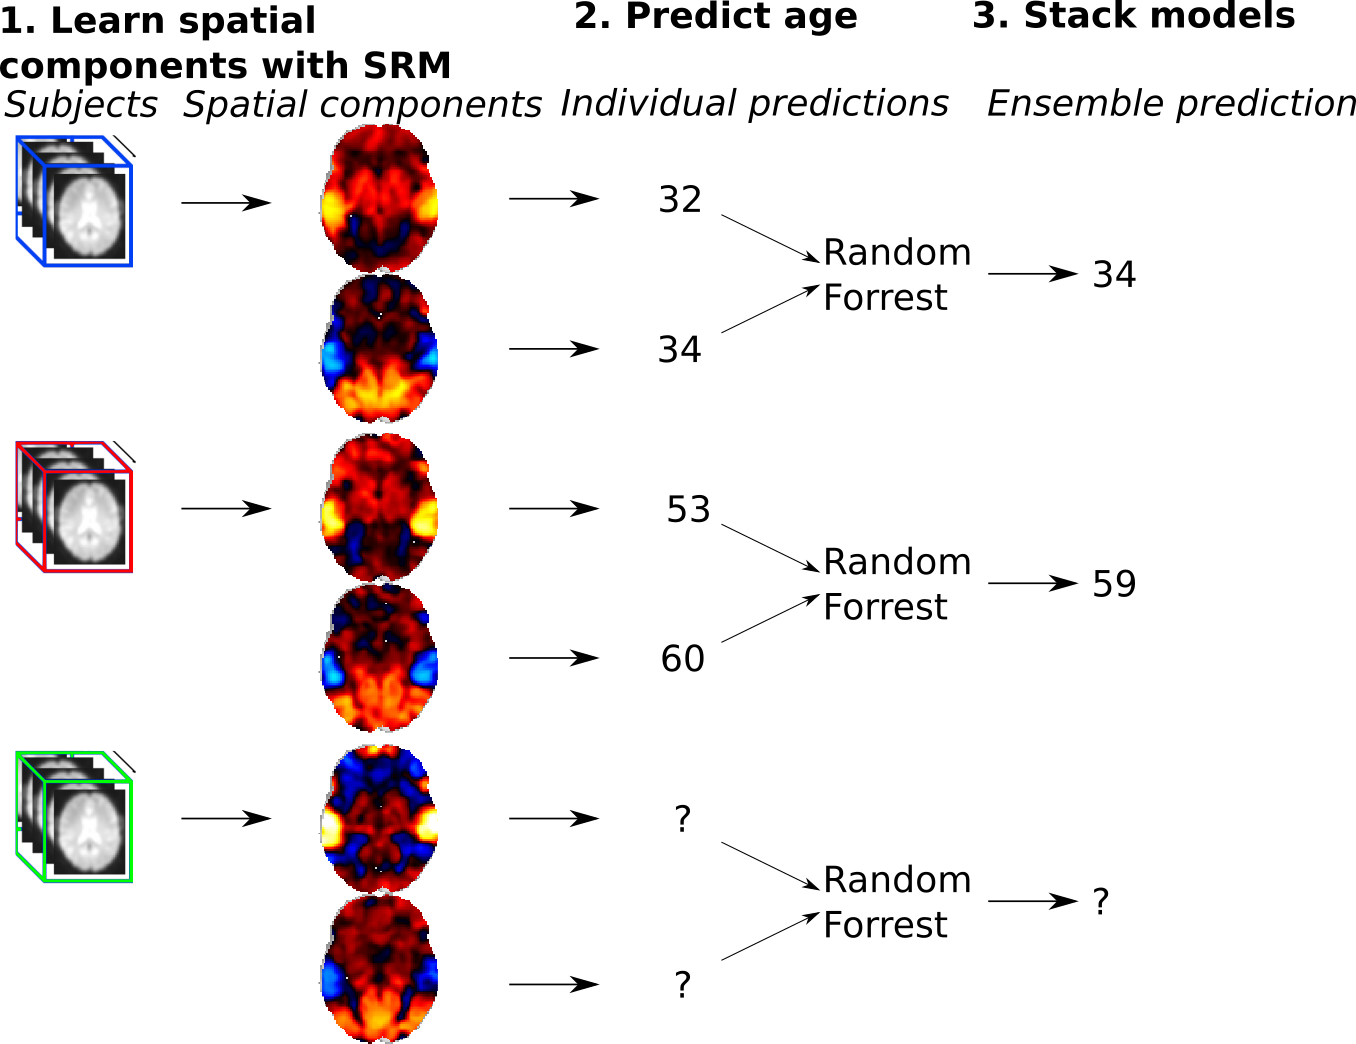
\includegraphics[scale=0.35]{figures/srm/conceptual_figure72.png}
\caption{\textbf{Experiment — Predict age from spatial components extracted using FastSRM}: We first learn the spatial components from fMRI data using SRM. We learn one Ridge model per spatial components to predict age across subjects. Then, these models are aggregated using a Random Forest (like in \cite{rahim2017joint}).} 
\label{fig:experiment_age_prediction}
\end{figure}


In order to assess which spatial components are most predictive of age, we
assess the feature importance via the Gini index defined in
\cite{breiman2001random} or \cite{louppe2013understanding} that measures the
relative reduction in Gini impurity brought by each feature.
%
Feature importance varies with different splits. We use the averaged feature
importance over the 5 splits of our pipeline and plot the 3 most important
spatial components according to this metric in Figure~\ref{fig:predict_age}.
These spatial components represent respectively 16\%, 12\% and 8\% of the total
feature importance and they highlight the the visual dorsal pathway, the
precuneus and the visual ventral pathway respectively. 
%
The fact that averaged spatial components are interpretable and meaningful allows us to study the influence of age on brain networks involved in movie-watching.
%
In Figure~\ref{fig:predict_age_interpretation}, we plot the most important spatial component averaged within groups of ages.
%
We see that these spatial components evolve with age allowing us to visually identify which regions are meaningful. 
%
It turns out that aging is mostly reflected in brain activity as a
fading of activity in the spatial correlates of movie watching,
particularly in the dorsal visual cortex.


\begin{figure}
\centering
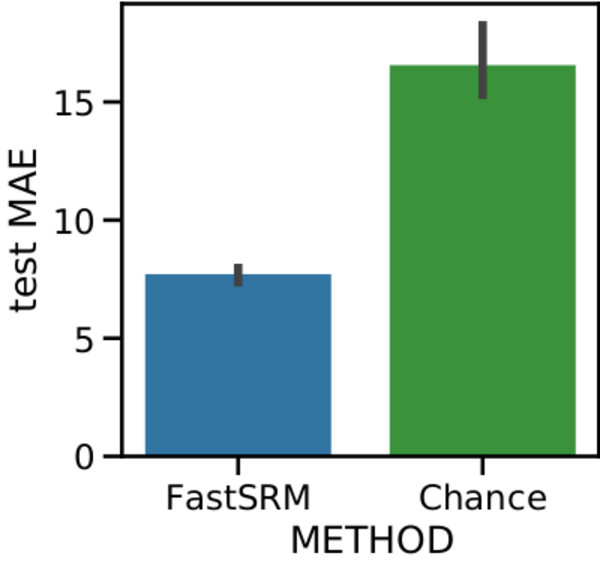
\includegraphics[scale=0.44]{figures/srm/predict_age.pdf}

\begin{tabular}{|c|c|c|}
	\hline
	Algorithm & Memory usage (in Go) & Fitting time (in minutes) \\
	\hline
	FastSRM & 18 & 9 \\
	ProbSRM & 178 & 2232 \\
	\hline
\end{tabular}

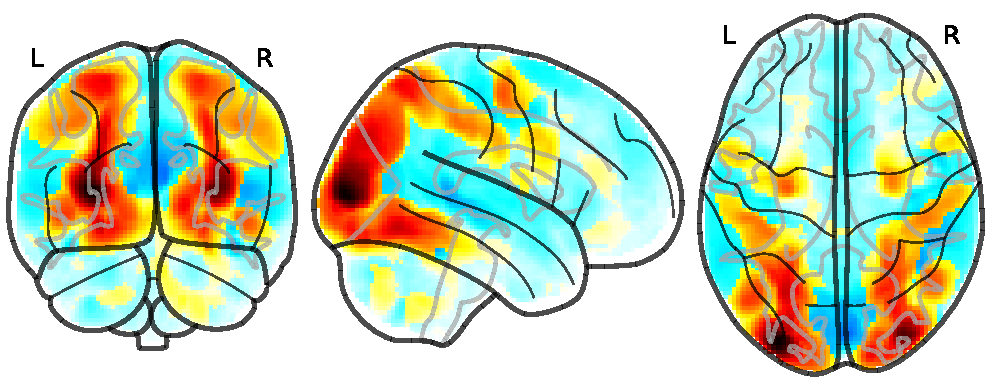
\includegraphics[scale=0.365]{./figures/srm/maps_feature_imp_0_16.pdf}
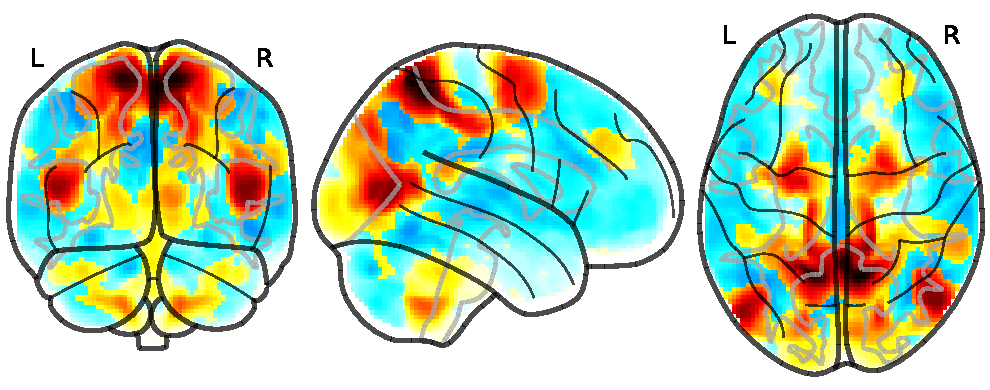
\includegraphics[scale=0.365]{./figures/srm/maps_feature_imp_0_12.pdf}
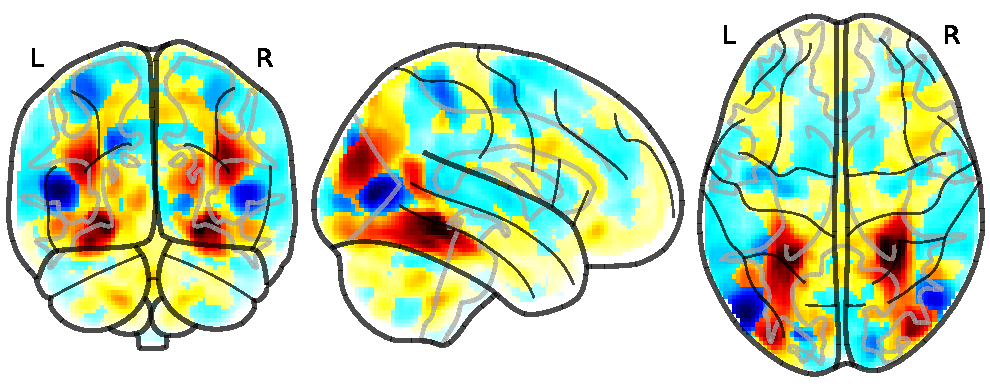
\includegraphics[scale=0.365]{./figures/srm/maps_feature_imp_0_08.pdf}

\caption{\textbf{Age prediction from spatial components}: (top) FastSRM predicts
  age with a better accuracy than chance resulting in a mean absolute error (MAE) of 7.5 years. (middle) FastSRM is more than 200x faster than ProbSRM and uses 10x less memory, hence it scales better than ProbSRM. (bottom) The three most important spatial components in terms of the reduction in Gini impurity they bring (see Gini importance or Feature importance in \cite{breiman2001random}, \cite{louppe2013understanding}). From top to bottom, the most important spatial component (feature importance: 16\%) highlights the visual dorsal pathway, the second most important spatial component (feature importance: 12\%) highlights the precuneus and the third most important spatial component (feature importance: 8\%) highlights the visual ventral pathway.} 
\label{fig:predict_age}
\end{figure}

\begin{figure}
\centering
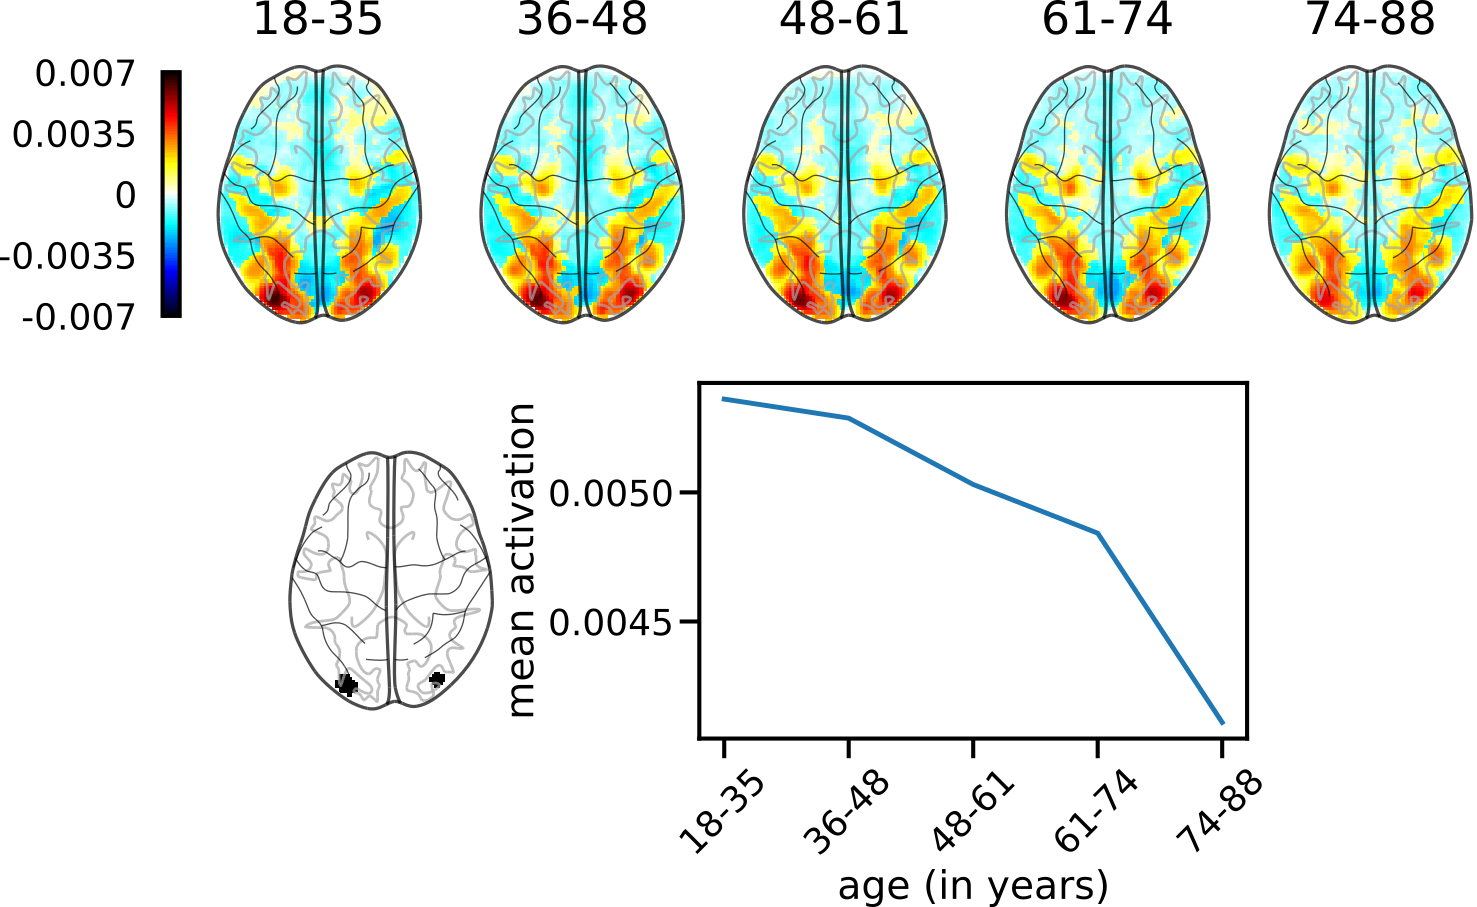
\includegraphics[scale=0.35]{figures/srm/feature_importance_age_prediction.png}
\caption{\textbf{Evolution of the most predictive spatial component with age}: (Top) Spatial component most predictive of age averaged within groups of different age (18-35, 36-48, 48-61, 61-74, 74-88). (Bottom) Mean activation in the region highlighted by the mask on the left. We see that the activity in the dorsal pathway decreases with age, which explains why this spatial component is a good predictor of age.}
\label{fig:predict_age_interpretation}
\end{figure}



\section{Conclusion}
As studies using naturalistic stimuli will tend to become more common and large
within and across subjects, we need scalable models in terms of computation time
and memory usage.
%
This is what FastSRM provides.
%
We show that while FastSRM is provably equivalent to its SRM counterpart in
terms of performance,  it has much lower fitting time and memory requirements.

FastSRM allows large scale analysis of fMRI data of subjects exposed to naturalistic stimuli. As one example of such analysis, we show that it can be used to predict age from movie-watching data. Interestingly, although FastSRM is an unsupervised model, it extracts meaningful networks and as such constitutes a practical way of studying subjects exposed to naturalistic stimuli.

We also show that individual information can be extracted from the fMRI activity when subjects are exposed to naturalistic stimuli. Our predictive model is reminiscent of that of \cite{bijsterbosch2018relationship}, that have shown that ICA components obtained from the decomposition of resting state data carry important information on individual characteristics. 
%
Our model inherits from all the weaknesses of SRM including the fact that
mixing matrices are assumed to be orthogonal which is rather unrealistic.
In later chapters, we see how this constraint can be released.
% The remaining difficulty with SRM is to interpret the spatio-temporal decomposition. Reverse correlation \cite{hasson2004intersubject} can be used to clarify the cognitive information captured in the shared response.